\documentclass[a4paper, 12pt]{article}
\usepackage{graphicx}
\graphicspath{ {/home/arian/Desktop/HEPIA/images/Sys-Emb/labo1} }
% Title information
\title{Journal de laboratoire}
\author{Arian Dervishaj}
\date{\today}

\begin{document}
\maketitle
\pagebreak

\section*{3. Exercices}
\subsection*{3.1 Mesure avec resistance}
\begin{enumerate}
    \item 97.0 $\Omega$
    \item \begin{itemize}
        \item $U = R*I \Longleftrightarrow I = U/R \Longleftrightarrow I = 5.00 / 97.0 = 0.052 A = 52 mA $
        \item $P = U * I = 5 * 0.052 = 0.26W$
        \end{itemize} 
    \item[4] La tension mesurée aux bornes de la resistance est de $4.88V$
    \item[5] La mesure du courant est de $48 mA$
\end{enumerate}

\subsection*{3.2 Résistance en série}
\begin{enumerate}
    \item Les deux sont de $97 \Omega$
    \item Oui
    \item 1ere : 23mA, 2ème : 23 mA
    \item \begin{itemize}
        \item $I = U/R \Longleftrightarrow I = 5.00 / 97.0 = 0.052 A = 52 mA $
        \item $P = U * I = 5 * 0.052 = 0.26W.$
        \end{itemize} 
\end{enumerate}

\subsection*{3.3 Résistance en parallèle}
\begin{enumerate}
    \item $97 \Omega$
    \item Le tension aux bornes de la première resistance est de 4.90V et la deuxième est de 4.93V
    \item $R_1 = 47.8mA$, $R_2 = 47.2mA$
    \item 
        \begin{itemize}
            \item $I = U/R \Longleftrightarrow I = 5.00 / 97.0 = 0.052 A = 52 mA$
            \item $P = U * I = 5 * 0.052 = 0.26W.$
        \end{itemize}
\end{enumerate}

\subsection*{3.4 Diode électroluminescente}
\begin{enumerate}
    \item[3] $R = 120 \Omega \\ U_{R} = 1.7V, \\ U_{Led} = 3.1 \\ U_{A}=5V \\ U_{R} + U_{Led} = 1.7 + 3.1 = 5 = U_{A}$
    \item[4] $I = 14.7mA$  
    \item[5] $R = 180 \Omega \\ U_{R} = 1.8V \\ U_{Led} = 3.3V \\ I = 10.4mA$
    \item[6] \begin{itemize}
        \item[c.] $  0mA \rightarrow 2V \\ 3V \rightarrow 1.3mA \\ 4V \rightarrow 5.8mA \\ 5V \rightarrow 11mA \\ 6V \rightarrow 15.5mA \\ 6.8V \rightarrow 20mA$
        \item[d.] Plus intensité est forte, plus la lumière est forte 
        \item[e.]   \begin{minipage}{0.6\textwidth}
                            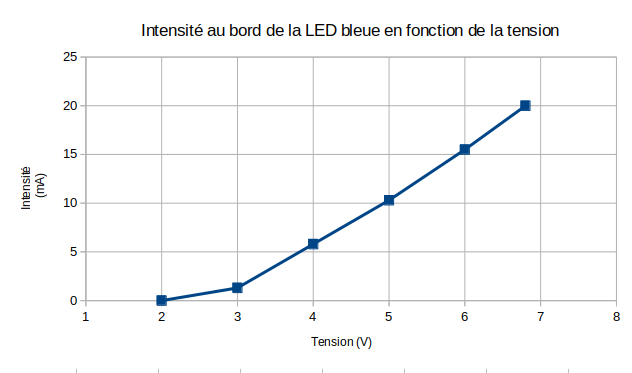
\includegraphics[scale=0.5]{Graphic_Labo1.png}
                    \end{minipage}
    \end{itemize} 
\end{enumerate}
\end{document}
